\documentclass[8pt]{beamer}
\usepackage[utf8]{inputenc}
\usepackage{xcolor}
\usepackage{colortbl}
\usepackage{epsfig}
% \usepackage{cancel}
\usepackage{ulem}
% \usepackage{threeparttable} % Joao Pela: 
\usepackage{amsmath}
\usepackage{hyperref}
\usepackage{siunitx}  % Allows easy x10^ for numbers
% \usepackage{appendixnumberbeamer}

\usetheme{Madrid}

\author[J. Pela]{João Pela}
\title{QCD VBF+MET samples for Run2 Update}
\institute[ICL]{Imperial College London}
\date{2015-04-28}

% The log drawn in the upper right corner.
\logo{\includegraphics[height=0.115\paperheight]{img/Logo_CMSICL.png}}

\begin{document}
\setlength{\unitlength}{1mm}

% ###################################################
\begin{frame}
  \titlepage
\end{frame}

% ###################################################
\begin{frame}{Introduction}

During Run I a set of QCD samples with VBF like jets and real MET was generated, which allowed:

\begin{block}
  
\begin{itemize}
  \item Understand real MET in QCD
  \item Indirectly ``determine the importance`` of fake MET events (which we were not modelling)
\end{itemize}

\end{block}

For Run II making such samples once again to be useful, but:

\begin{block}

\begin{itemize}
  \item Is it possible (cross section increase significantly)?
  \item What are the costs (CPU time and storage)?
  \item Is it possible to have samples what include fake MET?
  \item What cuts to apply? And what is the physics toll?
\end{itemize}
  
\end{block}

\end{frame}

% ###################################################
\begin{frame}{Run I samples}

As a reminder here are the generator cuts used to generate the run I QCD samples.

\begin{block}{MC Filter: Vectorial sum of neutrino $E_T$}

\begin{itemize}
  \item $\sum E_\perp(\vec{\nu}) > 40$ $GeV$
\end{itemize}

\end{block}

\begin{block}{MC Filter: Dijet Filter (AK5 GenJet no $\mu$)}

\begin{itemize}
  \item Select jets with:
  \begin{itemize}
    \item $p_\perp>20$ $GeV$
    \item $|\eta|<5.0$
  \end{itemize}
  \item From selected jets at least one pair with:
  \begin{itemize}
    \item $m_{jj}>700$ $GeV$
    \item $\Delta\eta>3.2$
  \end{itemize}    
\end{itemize}

\end{block}

\end{frame}

% ###################################################
\begin{frame}{Filters and goals}
 
Steps where filters can (easily...) be inserted:

\begin{block}

\begin{itemize}
 \item Monte Carlo Generation
 \item Level 1 Trigger
 \item High Level Trigger
 \item Offline
\end{itemize}

\end{block}
 
Goals for this samples:

\begin{block}

\begin{itemize}
  \item Avoid: Generator MET cut, (also pick fake MET events).
  \item Samples should be of similar size to the inclusive QCD samples.
  \item $\Delta\phi(jet-jet)$ cuts should be avoided if possible (Run I analysis uses $\Delta\phi(jet-jet)$ cut for data-driven QCD estimation).
\end{itemize}

\end{block}

\end{frame}


% ###################################################
\begin{frame}{Cross Sections}

\begin{block}{Cross Section for some QCD $p_\perp$ hats}
  
\begin{table}[htp]
\centering

\begin{tabular}{|c|c|c|c|}
\hline
 & \multicolumn{3}{c|}{Cross Section [pb]} \\
\hline
$p_\perp$ hat [GeV] & 8 TeV & 13 TeV & Change \\
\hline
\hline
30-50   & 66285328      & 161500000.   & +243.6\% \\
50-80   &  8148778.0    &  22110000.   & +271.3\% \\
80-120  &  1033680.0    &   3000114.3  & +290.2\% \\
120-170 &   156293.3    &    493200.   & +315.6\% \\
170-300 &    34138.15   &    120300.   & +352.4\% \\
300-470 &     1759.549  &      7475.   & +424.8\% \\
470-600 &      113.8791 &       587.1  & +515.5\% \\
600-800 &       26.99   &       167.   & +618.7\% \\
\hline
\end{tabular}

\end{table}



\end{block}
  
As expected cross section for the this QCD $p_\perp$ hats increase significantly from 8 to 13 TeV.
  
\end{frame}

% ###################################################
\begin{frame}{Events for 10 and 30 $fb^-1$}

\begin{block}

\begin{table}
\centering

\begin{tabular}{|c|c|c|c|}
\hline
pT Hat &  X-Section (pb) &  10 fb-1 & 30 fb-1 \\
\hline
\hline
  30-50 & \num{1.62E+08} & \num{1.62E+12} & \num{4.85E+12} \\
  50-80 & \num{2.21E+07} & \num{2.21E+11} & \num{6.63E+11} \\
 80-120 & \num{3.00E+06} & \num{3.00E+10} & \num{9.00E+10} \\
120-170 & \num{4.93E+05} & \num{4.93E+09} & \num{1.48E+10} \\
170-300 & \num{1.20E+05} & \num{1.20E+09} & \num{3.61E+09} \\
300-470 & \num{7.48E+03} & \num{7.48E+07} & \num{2.24E+08} \\
470-600 &          587.1 & \num{5.87E+06} & \num{1.76E+07} \\
600-800 &            167 & \num{1.67E+06} & \num{5.01E+06} \\
\hline
\end{tabular}


\caption{Quantity of event for each of the studied QCD $p_\perp$ hats for 10 and 30 $fb^-1$ of integrated luminosity.}
\label{table_QCD_RunII_EventsIntegratedLuminsity}
\end{table} 


\end{block}
  
Knowing that the current QCD samples sizes (470-600: 2.9M and 600-800: 2.8M) we can conclude:
\begin{itemize}
  \item For 10 $fb^-1$ we need to simulate up to bin 470-600
  \item For 30 $fb^-1$ we need to simulate up to bin 600-800
\end{itemize}

\end{frame}


% ###################################################
\begin{frame}{Unfiltered production: Hardware}

A single job for the whole simulation chain for 100 events was submitted to CERN lxbatch.
\begin{itemize}
  \item GEN, SIM, DIGI, L1, DIGI2RAW, HLT:GRun
  \item RAW2DIGI, L1Reco, RECO
\end{itemize}

\begin{block}{Hardware characteristics}
 
\begin{table}[htp]
\centering

\begin{tabular}{|c|c|l|c|c|}
\hline
\multicolumn{2}{|c|}{$p_\perp$ hat} & \multicolumn{3}{c|}{System Characteristics} \\
\hline
Min & Max & CPU Model & Core & RAM (kB) \\
\hline
\hline
 30 &  50 & Intel Core i7 9xx                         & 16 & 24023052 \\
 50 &  80 & Intel(R) Xeon(R) CPU E5-2650 v2 @ 2.60GHz & 32 & 62533844 \\
 80 & 120 & AMD Opteron(TM) Processor 6276            & 32 & 62533828 \\
120 & 170 & Intel(R) Xeon(R) CPU E5-2650 v2 @ 2.60GHz &  8 & 62533828 \\
170 & 300 & AMD Opteron(TM) Processor 6276            & 32 & 62533828 \\
300 & 470 & Intel(R) Xeon(R) CPU E5-2650 v2 @ 2.60GHz & 16 & 31225964 \\
470 & 600 & Intel(R) Xeon(R) CPU E5-2650 v2 @ 2.60GHz & 32 & 62533844 \\
600 & 800 & Intel Core i7 9xx                         & 16 & 24023052 \\
\hline	
\end{tabular}

\label{table_QCD_ProdUnfiltered_Hardware}
\end{table}


\end{block}

To note that at lxplus (which I will assume is representative of the grid resources) machines can be very different in terms of CPU and number of cores. Differences were observed in CPU time between machines executing exactly the same code of +50\% (sometimes as high as +100\%).

\end{frame}

% ###################################################
\begin{frame}{Unfiltered production: Step 1}
 
Here are the statistics for the step 1 computing
 
\begin{block}{Step 1 statistics}

\begin{table}[htp]
\centering

\begin{tabular}{|c|c||c|c||c|c|c|c||c|c|}
\hline
\multicolumn{2}{|c|}{$p_\perp$ hat} & \multicolumn{2}{|c||}{Job Times} & \multicolumn{4}{c||}{CPU Times} & \multicolumn{2}{c|}{Size (MB)} \\
\hline
Min & Max & Total & Avg Event & Total & Total Event & Avg Event & Non-Event   & Job & Avg Event \\
\hline
\hline
 30 &  50 & 9985.93 & 99.8593 & 7520.65 & 7394.73 & 73.9473 & 125.92 & 128 & 1.28 \\
 50 &  80 & 10769.5 & 107.695 & 7462.92 & 7369.9  & 107.695 &  93.02 & 132 & 1.32 \\
 80 & 120 & 16576.5 & 165.765 & 12902   & 12739.3 & 127.393 &  162.7 & 144 & 1.44 \\
120 & 170 & 10942.9 & 109.429 & 8302.49 & 8216.92 & 82.1692 &  85.57 & 152 & 1.52 \\
170 & 300 & 18225.8 & 182.258 & 14636.6 & 14475.7 & 144.757 &  160.9 & 165 & 1.65 \\
300 & 470 & 13346.1 & 133.461 & 11611.5 & 11523.6 & 115.236 &   87.9 & 177 & 1.77 \\
470 & 600 & 15774.7 & 157.747 & 13511.4 & 13413.7 & 134.137 &   97.7 & 189 & 1.89 \\
600 & 800 & 16422.1 & 164.221 & 15851.5 & 15726.5 & 157.265 &    125 & 192 & 1.92 \\
\hline
\hline
\multicolumn{2}{|l|}{Average} & 14005 & 140.05 & 11474.9 & 11357.5 & 117.8 & 117.3 &  &  \\
\hline
\end{tabular}

\caption{Step 1}
\label{table_QCD_ProdUnfiltered_Step1}
\end{table}

% -rw-r--r--. 1 pela zh 128M Apr 12 03:12 QCD_Pt-30to50_step1.root
% -rw-r--r--. 1 pela zh 132M Apr 12 03:24 QCD_Pt-50to80_step1.root
% -rw-r--r--. 1 pela zh 144M Apr 12 05:01 QCD_Pt-80to120_step1.root
% -rw-r--r--. 1 pela zh 152M Apr 12 03:28 QCD_Pt-120to170_step1.root
% -rw-r--r--. 1 pela zh 165M Apr 12 05:28 QCD_Pt-170to300_step1.root
% -rw-r--r--. 1 pela zh 177M Apr 12 04:06 QCD_Pt-300to470_step1.root
% -rw-r--r--. 1 pela zh 189M Apr 12 04:48 QCD_Pt-470to600_step1.root
% -rw-r--r--. 1 pela zh 192M Apr 12 04:59 QCD_Pt-600to800_step1.root


% -rw-r--r--. 1 pela zh  30M Apr 12 03:34 QCD_Pt-30to50_step2.root
% -rw-r--r--. 1 pela zh  32M Apr 12 03:51 QCD_Pt-50to80_step2.root
% -rw-r--r--. 1 pela zh  34M Apr 12 05:50 QCD_Pt-80to120_step2.root
% -rw-r--r--. 1 pela zh  35M Apr 12 03:56 QCD_Pt-120to170_step2.root
% -rw-r--r--. 1 pela zh  37M Apr 12 06:22 QCD_Pt-170to300_step2.root
% -rw-r--r--. 1 pela zh  39M Apr 12 05:04 QCD_Pt-300to470_step2.root
% -rw-r--r--. 1 pela zh  40M Apr 12 05:37 QCD_Pt-470to600_step2.root
% -rw-r--r--. 1 pela zh  41M Apr 12 05:49 QCD_Pt-600to800_step2.root



\end{block}

Some conclusions
\begin{itemize}
  \item It would be impossible to process every single event, it would take several millennia on a single CPU. We need some kind of gen filter.
  \item On average events take between 1 and 3 minutes to go over the whole step.
  \item Event size is under 2 MB (this is normal) and increases with $p_\perp$ hat.
\end{itemize}

NOTE: I am including PU at average 30 interactions.

\end{frame}

% ###################################################
\begin{frame}{Unfiltered production: Step 2}
 
Here are the statistics for the step 2 computing
 
\begin{block}{Step 2 statistics}

\begin{table}[htp]
\centering

\resizebox{\linewidth}{!}{
\begin{tabular}{|c||c|c|c|c||c|c|}
\hline
 & \multicolumn{4}{c||}{CPU Times} &  \\
\hline
$p_\perp$ hat & Total & Total Event & Avg Event & Non-Event   & Ev. Size (MB) \\
\hline
\hline
  30-50 & 1074.55 & 1023.63 & 10.2363 & 50.92 & 0.30 \\
  50-80 & 1163.04 & 1108.85 & 11.0885 & 54.19 & 0.32 \\
 80-120 & 2395.97 & 2308.39 & 23.0839 & 87.58 & 0.34 \\
120-170 & 1276.21 & 1232.36 & 12.3236 & 43.85 & 0.35 \\
170-300 & 2632.94 & 2548.5  & 25.485  & 84.44 & 0.37 \\
300-470 & 1832.55 & 1776.45 & 17.7645 & 56.1  & 0.39 \\
470-600 & 2130.65 & 2055.35 & 20.5535 & 75.3  & 0.40 \\
600-800 & 2726.66 & 2658.05 & 26.5805 & 68.61 & 0.41 \\
\hline
\hline
Average & 2269.0 & 1838.9 & 18.4 & 65.1 & 0.36 \\
\hline
\end{tabular}
}

\label{table_QCD_ProdUnfiltered_Step2}
\end{table}


\end{block}

Some conclusions
\begin{itemize}
  \item This step will not be a problem since it is after the selection
  \item Event size is under 0.5 MB (this is normal) and increases with $p_\perp$ hat.
\end{itemize}


\end{frame}

% ###################################################
\begin{frame}{First working point}

\begin{center}
GenJets only ($p_\perp>50$, $|eta|<4.75$, $\Delta_{\eta}>3.5$, $\Delta_{\phi}<1.5$, $m_{jj}>1000$)
\end{center}

\begin{block}{Step 1 statistics: 1M events}

\resizebox{\linewidth}{!}{
\begin{tabular}{|c||c|c|c|c||c|c|c|}
\hline
 & \multicolumn{4}{c||}{CPU Times} &  \\
\hline
$p_\perp$ hat & Passed & Filter Eff Event & Total Filter &  Ev Total S1 CPU (s)  & S1 5k CPU (h) & S1 5k CPU (d) \\
\hline
\hline
  30-50 & 6     & \num{6.00E-06} & \num{9.69E+06} & \num{7.17E+08} & 39.81  & 1.66 \\
  50-80 & 417   & \num{4.17E-04} & \num{9.22E+07} & \num{9.93E+09} & 551.63 & 22.98 \\
 80-120 & 3204  & \num{3.20E-03} & \num{9.61E+07} & \num{1.22E+10} & 680.30 & 28.35 \\
120-170 & 8857  & \num{8.86E-03} & \num{4.37E+07} & \num{3.59E+09} & 199.41 & 8.31 \\
170-300 & 18828 & \num{1.88E-02} & \num{2.27E+07} & \num{3.28E+09} & 182.15 & 7.59 \\
300-470 & 36953 & \num{3.70E-02} & \num{2.76E+06} & \num{3.18E+08} & 17.68  & 0.74 \\
470-600 & 46455 & \num{4.65E-02} & \num{2.73E+05} & \num{3.66E+07} & 2.03   & 0.08 \\
600-800 & 47430 & \num{4.74E-02} & \num{7.92E+04} & \num{1.25E+07} & 0.69   & 0.03 \\
\hline
\hline
\multicolumn{4}{|l|}{Total} & \num{3.01E+10} & 1673.71 & 69.74 \\
\hline
\end{tabular}
}

\begin{itemize}
  \item NOTE 1: 10x the statistics of last week!
  \item NOTE 2: Time values do not include generator level times just reco times (should be dominant for higher $p_\perp$ hats.
\end{itemize}

\end{block}

We could make this samples with 5k CPU in about 2 months, can be done privately with some work, but can be done easily by central production!

\end{frame}

% ###################################################
\begin{frame}{Other working points}

\begin{block}{Filter statistics}

\resizebox{\linewidth}{!}{
\begin{tabular}{|l||c|c|c||l|}
\hline
 & \multicolumn{3}{c||}{CPU Times} &  \\
\hline
Filter &  Ev Total S1 CPU (s)  & S1 5k CPU (h) & S1 5k CPU (d) & Note \\
\hline
\hline
Pt20\_Eta5p0\_DEta3p2\_Mjj700            & 4.03E+12 & 223652.83 & 9318.87 & Same as Run I without Generator MET \\
\hline
Pt50\_Eta4p75\_DEta3p5\_Dphi1p5\_Mjj1000 & 3.01E+10 &   1673.71 &   69.74 & Current working point \\
\hline
Pt40\_Eta4p75\_DEta3p5\_Mjj600           & 1.00E+12 &  55531.17 & 2313.80 & Same as new HLT path \\
Pt40\_Eta4p75\_DEta3p5\_Dphi1p5\_Mjj600  & 1.90E+11 &  10539.90 &  439.16 & Same as new HLT path + $\Delta\phi$ \\
\hline
Pt40\_Eta4p75\_DEta3p5\_Dphi1p5\_Mjj1000 & 6.87E+10 &   3816.26 &  159.01 & Lower 10 GeV Dijet $p_\perp$ \\
\hline
Pt50\_Eta4p75\_DEta3p5\_Dphi2p0\_Mjj1000 & 4.10E+10 &   2280.27 &   95.01 & +0.5 $\Delta\phi$ cut \\
Pt50\_Eta4p75\_DEta3p5\_Dphi2p5\_Mjj1000 & 6.24E+10 &   3467.57 &  144.48 & +1.0 $\Delta\phi$ cut \\
Pt50\_Eta4p75\_DEta3p5\_Mjj1000          & 2.34E+11 &  13025.79 &  542.74 & No $\Delta\phi$ cut \\
\hline
\hline
\end{tabular}
}
  
\end{block}

\begin{itemize}
  \item Changing any studied parameter increases greatly the time to be spent generating 
  \item Touching $\Delta\phi$ increases processing time about 1 month per 0.5 relaxation
  \item Currently proposed working point same as last week
\end{itemize}

\end{frame}

% ###################################################
\begin{frame}{Offline Filter Efficiency}

For working point $p_\perp>50$, $|eta|<4.75$, $\Delta_{\eta}>3.5$, $\Delta_{\phi}<1.5$, $m_{jj}>1000$

\begin{block}{Level 1 MET}

\begin{columns}

\column[t]{0.45\linewidth}  

  \centering
  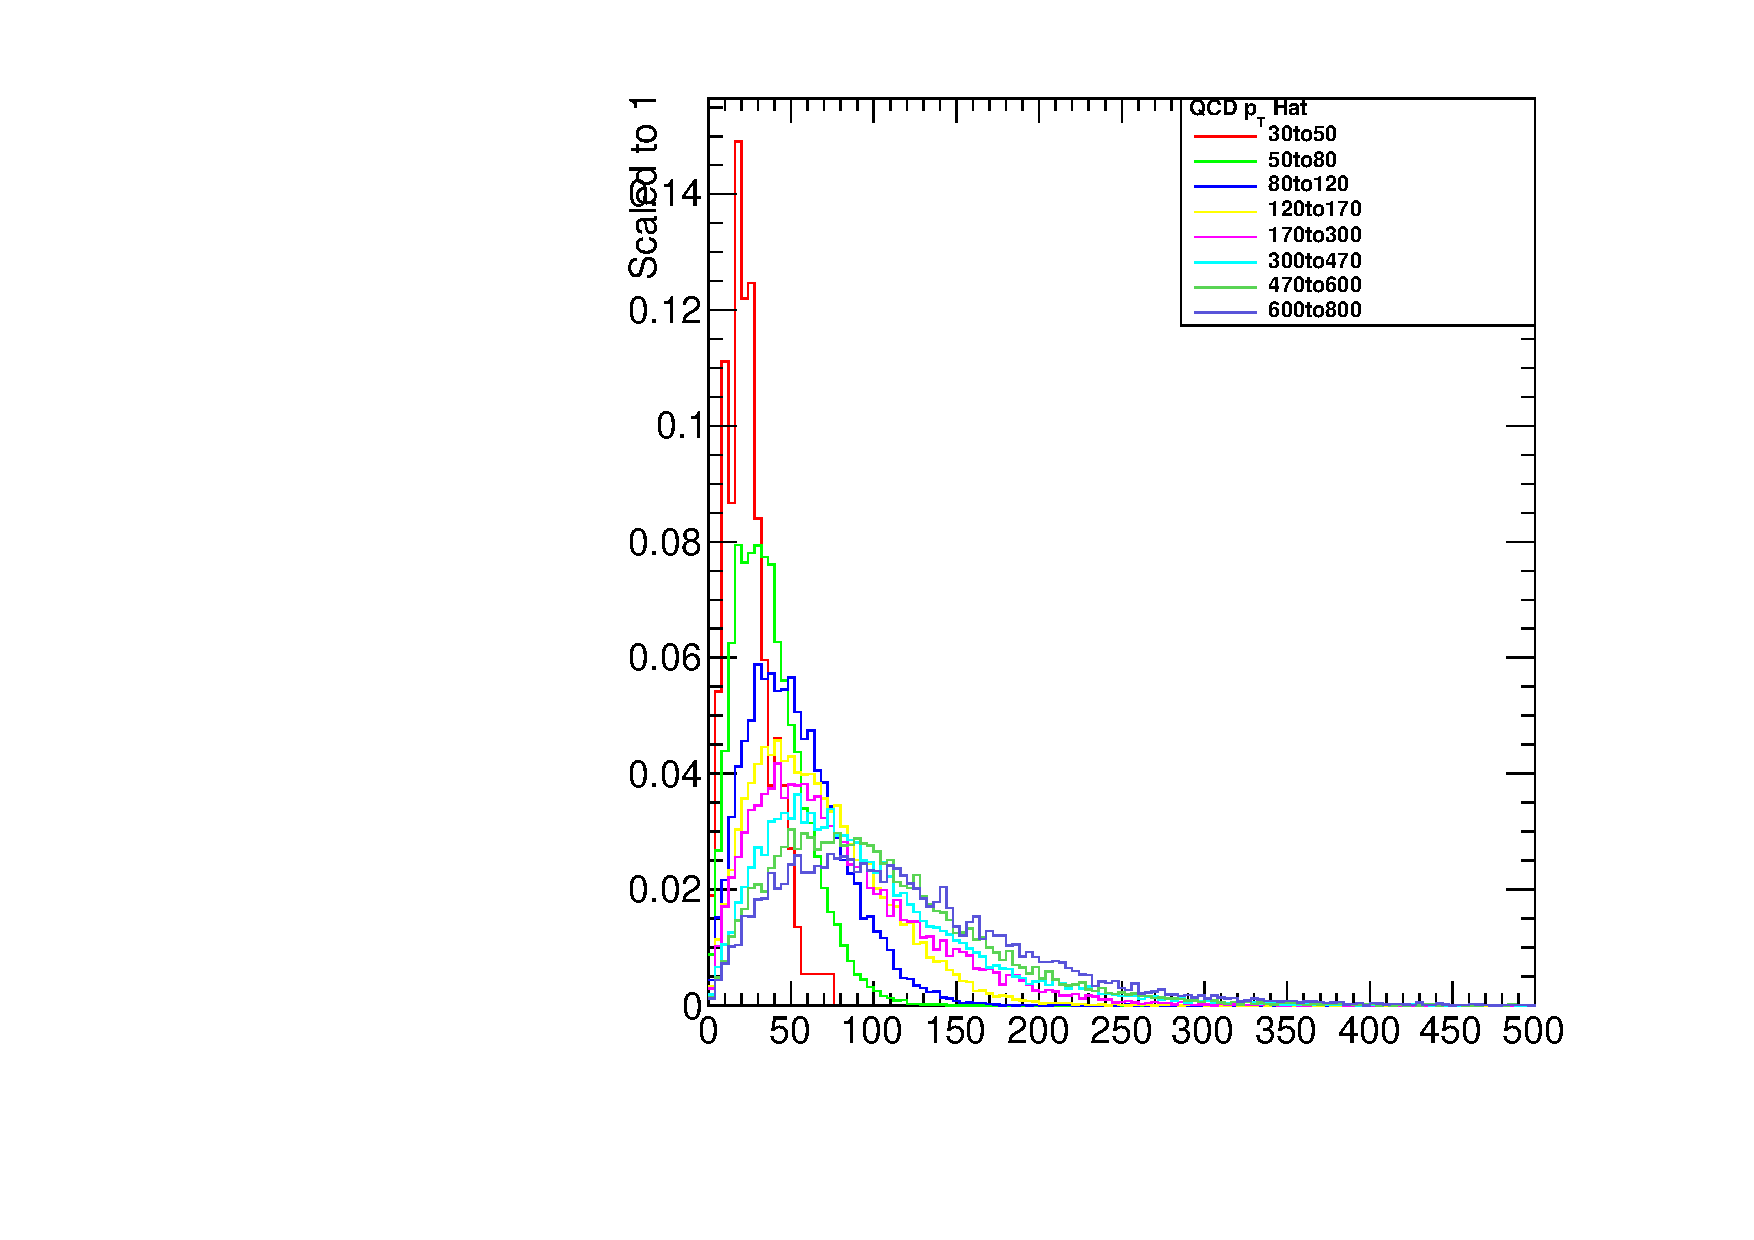
\includegraphics[width=0.8\linewidth]{img/L1Extra_MET.pdf}

\column[t]{0.45\linewidth}  

\begin{itemize}
  \item Here L1 MET is the one the comes from this CMSSW version, its NOT the latest greatest.
  \item We can see that many events have high L1 MET (much more than just real MET)
\end{itemize}

\end{columns}
  
\end{block}


\end{frame}

% ###################################################
\begin{frame}{Some new numbers}

\begin{block}{Level 1 MET}

\begin{itemize}
  \item L1T MET $ > 40$: 1.48E+08 (biggest sample 80-120 with 6.01E+07)
  \item L1T MET $ > 70$: 6.13E+07 (biggest sample 80-120 with 2.39E+07)
\end{itemize}

\end{block}

\begin{center}
60M for 8 samples is not unreasonable!
\end{center}

\end{frame}

% ###################################################
\begin{frame}{HLT PFMET170}

\begin{block}{Efficiency}

\centering
\begin{tabular}{|c||c|c|c|}
\hline
$p_\perp$ hat & Generated & Passed & Filter Eff  \\
\hline
\hline                                   
  30-50 &   80000000    &   0 & 0        \\
  50-80 &   20000000    &   0 & 0        \\
 80-120 &      3800000  &   0 & 0        \\
120-170 & 2400000       &   0 & 0        \\
170-300 &  700000       &   8 & 0.000011 \\
300-470 &   460000      &  32 & 0.000070 \\
470-600 &   320000      & 112 & 0.000350 \\
600-800 &      270000   & 194 & 0.000719 \\
\hline
\hline
\end{tabular}

\end{block}
  
\begin{itemize}
  \item Most events are killed and we now have dedicated path for this
\end{itemize}
  
\end{frame}


% ###################################################
\begin{frame}{Summary}
 
\begin{block}{Summary:}
 
\begin{itemize}
  \item Found a working point with is feasible with no MET cut at generator level with the caveat that it has a delta phi cut.
  \item A document including all the information is being written and will be sent around soon.
\end{itemize}

\end{block}

\begin{block}{Next steps:}
 
\begin{itemize}
  \item Study decrease of $m_{jj}$ and $\Delta\eta$ (done not digested)
  \item Finish offline efficiency study
\end{itemize}

\end{block}

\end{frame}

\end{document}
